%%%%%%%%%%%%%%%%%%%%%%%%%%%%%%%%%%%%%%%%%
% Beamer Presentation
% LaTeX Template
% Version 1.0 (10/11/12)
%
% This template has been downloaded from:
% http://www.LaTeXTemplates.com
%
% License:
% CC BY-NC-SA 3.0 (http://creativecommons.org/licenses/by-nc-sa/3.0/)
%
%%%%%%%%%%%%%%%%%%%%%%%%%%%%%%%%%%%%%%%%%

%----------------------------------------------------------------------------------------
%	PACKAGES AND THEMES
%----------------------------------------------------------------------------------------

\documentclass{beamer}

\mode<presentation> {

% The Beamer class comes with a number of default slide themes
% which change the colors and layouts of slides. Below this is a list
% of all the themes, uncomment each in turn to see what they look like.

%\usetheme{default}
%\usetheme{AnnArbor}
%\usetheme{Antibes}
%\usetheme{Bergen}
%\usetheme{Berkeley}
%\usetheme{Berlin}
%\usetheme{Boadilla}
%\usetheme{CambridgeUS}
%\usetheme{Copenhagen}
%\usetheme{Darmstadt}
%\usetheme{Dresden}
%\usetheme{Frankfurt}
%\usetheme{Goettingen}
%\usetheme{Hannover}
%\usetheme{Ilmenau}
%\usetheme{JuanLesPins}
%\usetheme{Luebeck}
%\usetheme{Madrid}
%\usetheme{Malmoe}
%\usetheme{Marburg}
%\usetheme{Montpellier}
%\usetheme{PaloAlto}
%\usetheme{Pittsburgh}
%\usetheme{Rochester}
\usetheme{Singapore}
%\usetheme{Szeged}
%\usetheme{Warsaw}

% As well as themes, the Beamer class has a number of color themes
% for any slide theme. Uncomment each of these in turn to see how it
% changes the colors of your current slide theme.

%\usecolortheme{albatross}
%\usecolortheme{beaver}
%\usecolortheme{beetle}
%\usecolortheme{crane}
%\usecolortheme{dolphin}
%\usecolortheme{dove}
%\usecolortheme{fly}
%\usecolortheme{lily}
%\usecolortheme{orchid}
%\usecolortheme{rose}
%\usecolortheme{seagull}
%\usecolortheme{seahorse}
%\usecolortheme{whale}
%\usecolortheme{wolverine}


%\setbeamertemplate{footline} % To remove the footer line in all slides uncomment this line
%\setbeamertemplate{footline}[page number] % To replace the footer line in all slides with a simple slide count uncomment this line

%\setbeamertemplate{navigation symbols}{} % To remove the navigation symbols from the bottom of all slides uncomment this line
}

\usepackage{graphicx} % Allows including images
\usepackage{booktabs} % Allows the use of \toprule, \midrule and \bottomrule in tables






%----------------------------------------------------------------------------------------
%	TITLE PAGE
%----------------------------------------------------------------------------------------

\title[Thesis]{HIGH PERFORMANCE OPPORTUNISTIC ROUTING ALGORITHMS FOR POWER CONSTRAINED NODES WITH MESSAGE DELIVERY DEADLINE IN SPARSE NETWORK ENVIRONMENT} % The short title appears at the bottom of every slide, the full title is only on the title page

\author{Jiradett Kerdsri} % Your name
\institute[SIIT] % Your institution as it will appear on the bottom of every slide, may be shorthand to save space
{
Sirindhorn International Institute of Technology,
Thammasat University \\ % Your institution for the title page
\medskip
\textit{jiradett.k@dti.or.th} % Your email address
}
\date{\today} % Date, can be changed to a custom date

\begin{document}

\begin{frame}
\titlepage % Print the title page as the first slide
\end{frame}

\begin{frame}
\frametitle{Overview} % Table of contents slide, comment this block out to remove it
\tableofcontents % Throughout your presentation, if you choose to use \section{} and \subsection{} commands, these will automatically be printed on this slide as an overview of your presentation
\end{frame}

%----------------------------------------------------------------------------------------
%	PRESENTATION SLIDES
%----------------------------------------------------------------------------------------

%------------------------------------------------
\section{Thesis Structure} % Sections can be created in order to organize your presentation into discrete blocks, all sections and subsections are automatically printed in the table of contents as an overview of the talk
%------------------------------------------------

%\subsection{Subsection Example} % A subsection can be created just before a set of slides with a common theme to further break down your presentation into chunks

\begin{frame}
\frametitle{Thesis Structure}

\begin{list}{-}{Chapter Title}
\item Signature Page 
\item  Acknowledgments 
\item  Abstract 
\item  Table of Contents 
\item  List of Figures 
\item  List of Tables 
\item List of Listings 
\item List of Acronyms
\end{list}

\begin{itemize}
\item Introduction 
\begin{itemize}
\item  Problem Statement 
\item  Objective and Scope 
\item  Proposed Approaches 
\item  Our Contributions 
\end{itemize}
\item  Background and Related Work 
\begin{itemize}
 	\item  Delay Tolerant Networks
	\item  Opportunistic Networks 
\end{itemize}
\end{itemize}
\end{frame}
%------------------------------------------------
\begin{frame}
	\frametitle{Thesis Structure}
	\begin{itemize}
\item  Dynamic Rendezvous based Routing Algorithm on Sparse Opportunistic Network Environment 
\begin{itemize}
	\item  Rendezvous Place  
	\item  Simulation Model and Results 
	\item  Summary of Contributions
\end{itemize}
\item  Data-wise Opportunistic Routing with Spatial Information  
\begin{itemize}
	\item  Data-wise Routing 
	\item  Simulation Model and Results 
	\item  Summary of Contributions 
\end{itemize}
\item  Conclusion and Future Work 
\begin{itemize}
	\item  Discussion
	\item  Conclusion 
	\item  Future Work
\end{itemize}
\item References
\item Appendix A: List of Publications
\end{itemize}
\end{frame}





%Existing works --> not applicable on some app
% Too my power
%Our Approaches
%
%
%
%
%
%

%------------------------------------------------
% What is OppNet --> Fix --> Traditional  --> Dynamic
\section{Opportunistic Network Overview}
\begin{frame}
	\frametitle{What is OppNet?}
	\begin{figure}
		\centering
		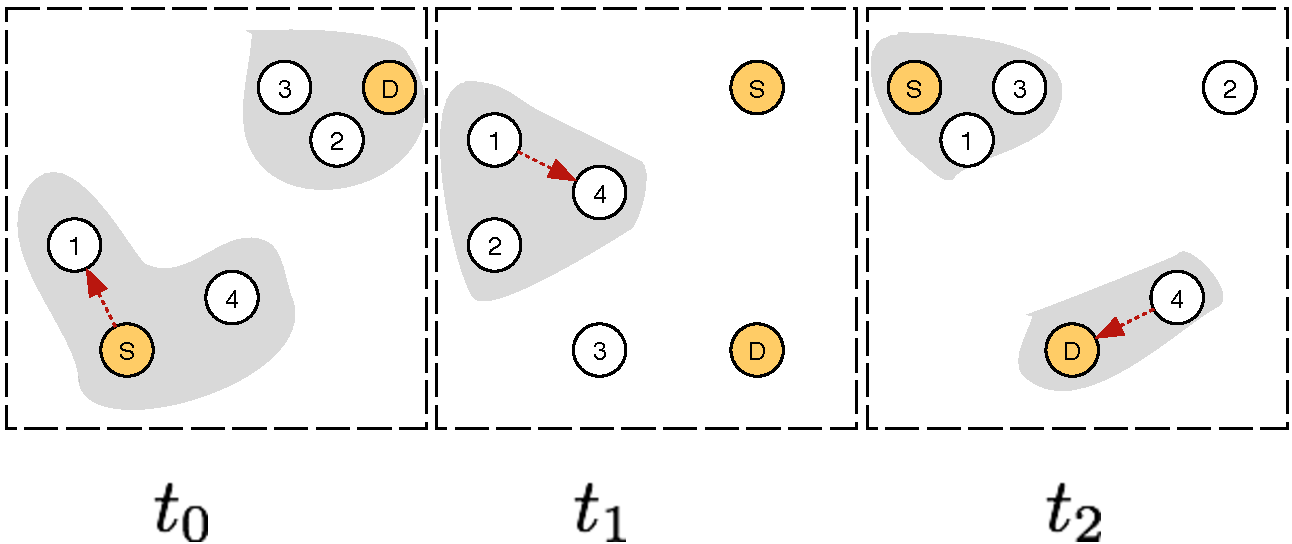
\includegraphics[width=0.7\linewidth]{Figures_Present/SFC}
		\caption{Store-Carry-Forward (SFC) protocol}
		\label{fig:SFC}
	\end{figure}
\begin{itemize}
	\item A challenge network where the nodes need to communicate with each other even either direct or indirect routes between them may not permanently exist due to the nodes’ random movement. 
	\item Using store- carry-forward paradigm 
\end{itemize}

\end{frame}
%------------------------------------------------
% Applications??
\begin{frame}
	\frametitle{Applications for OppNet}
	
	\begin{block}{Wildlife Monitoring}
		ZebraNet \cite{zebranet:2004}, SWIM \cite{Small2003} 
	\end{block}
	
	\begin{block}{Battlefield Network}
		Military tactical networks \cite{Scott2005} \cite{Kerdsri2013} 
	\end{block}
	
	\begin{block}{Disaster Monitoring Network}
		%find one to put in here
	\end{block}

\end{frame}


%------------------------------------------------
\section{Existing Works}
%------------------------------------------------
\begin{frame}
	\frametitle{Literatures Review}
	\begin{figure}
		\centering
		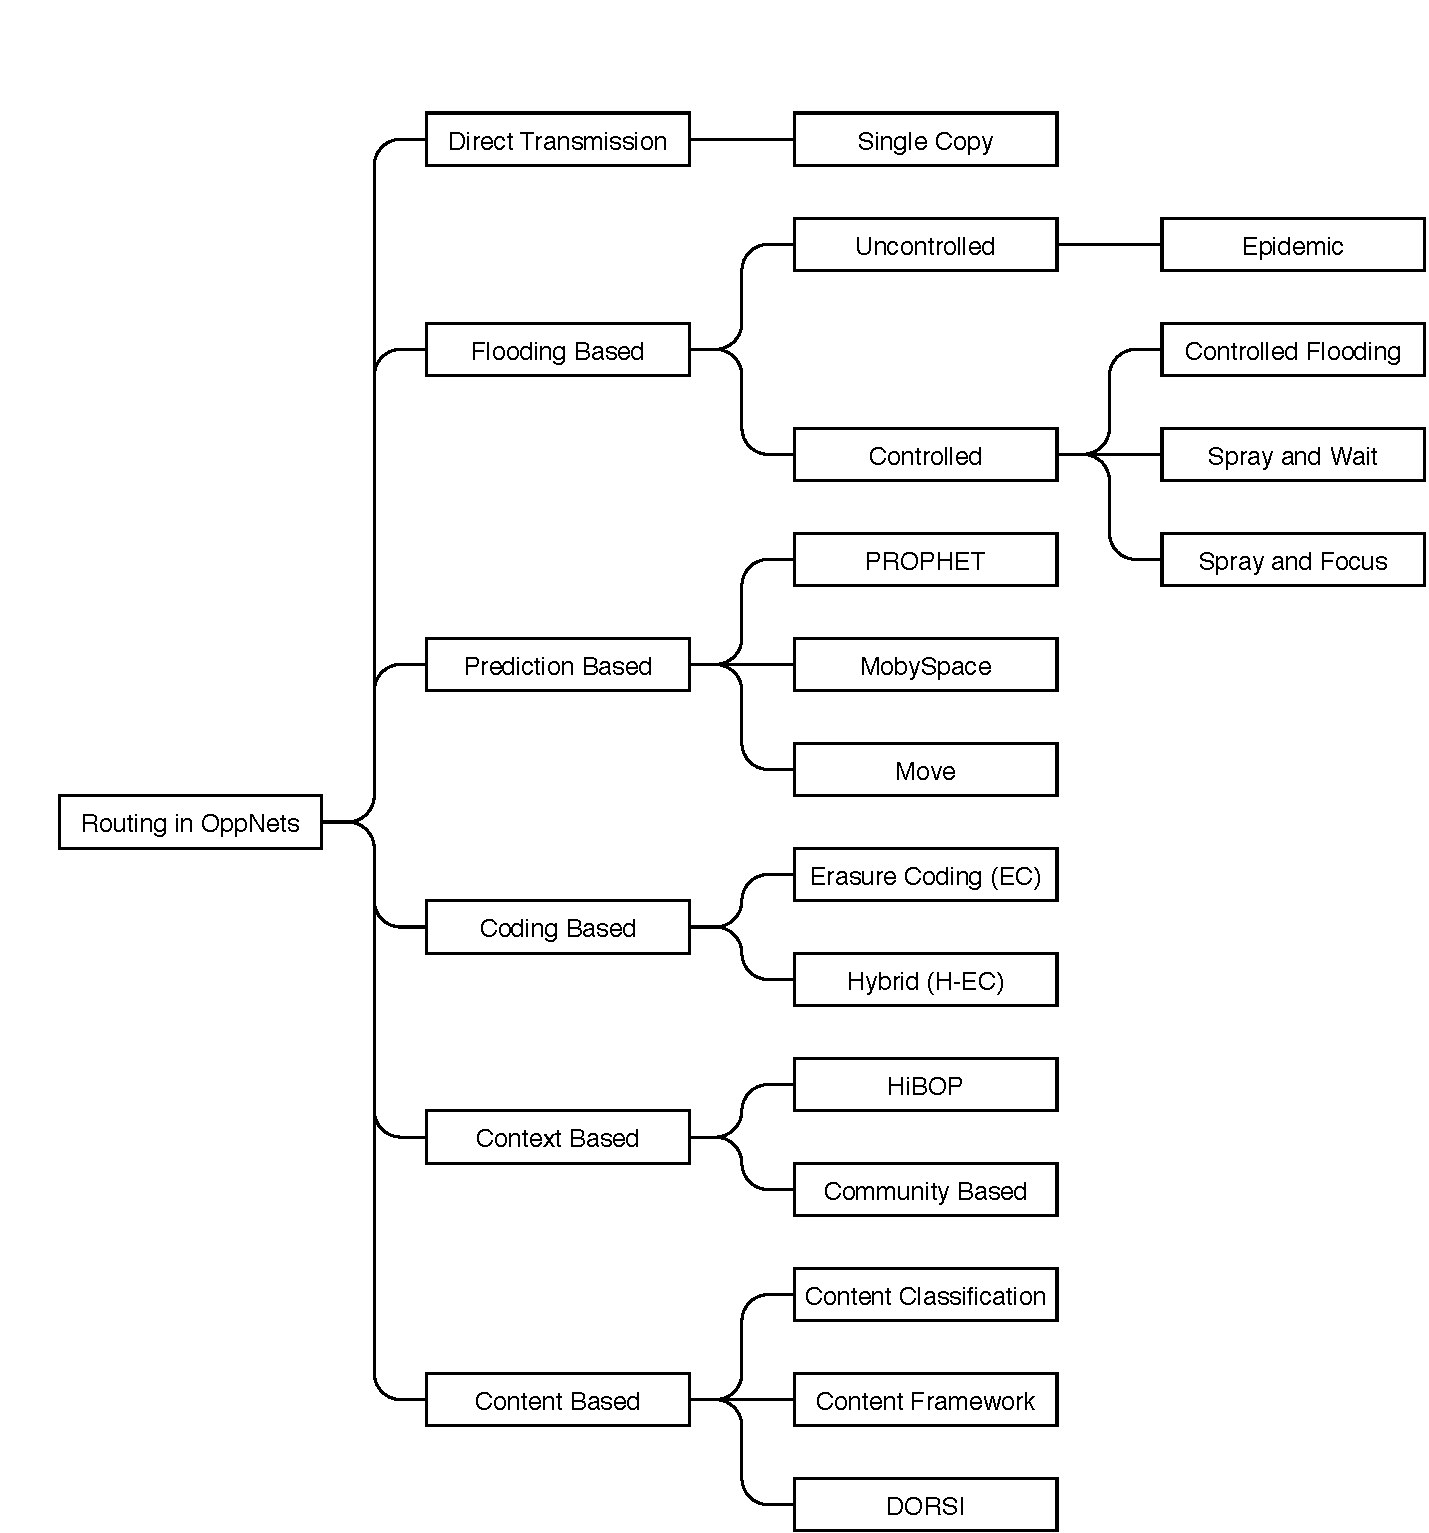
\includegraphics[width=0.5\linewidth]{Figures_Present/RoutingInOppNets}
		\caption{Diagram of Existing OppNet Routing}
		\label{fig:RoutingInOppNets}
	\end{figure}
	
\end{frame}


%------------------------------------------------
\section{Problem Statement}
%------------------------------------------------
%Problem --> Low delivery ratio
\begin{frame}
\frametitle{Problem Statement}


\begin{itemize}
\item Existing routing algorithms impractical on some applications
\item In this store-carry-forward paradigm, the network suffers the decreasing of performance in the insufficient collaborating nodes environment \cite{6196145,Spyropoulos2010}
\item Low delivery ratio in sparse network environment
\item Limited power resource 

\end{itemize}
\end{frame}


\begin{frame}
	\frametitle{Proposed Approaches}
	\begin{itemize}
		\item Dynamic Rendezvous based Routing Algorithm on Sparse Opportunistic Network Environment 
	
		
		\item DORSI: Data-wise Opportunistic Routing with Spatial Information
		
		
	\end{itemize}
\end{frame}

%------------------------------------------------
\section{Dynamic Rendezvous based Routing Algorithm on Sparse Opportunistic Network Environment}
%------------------------------------------------
\begin{frame}
	\frametitle{Rendezvous Based OppNet System Model}
	\begin{figure}
\centering
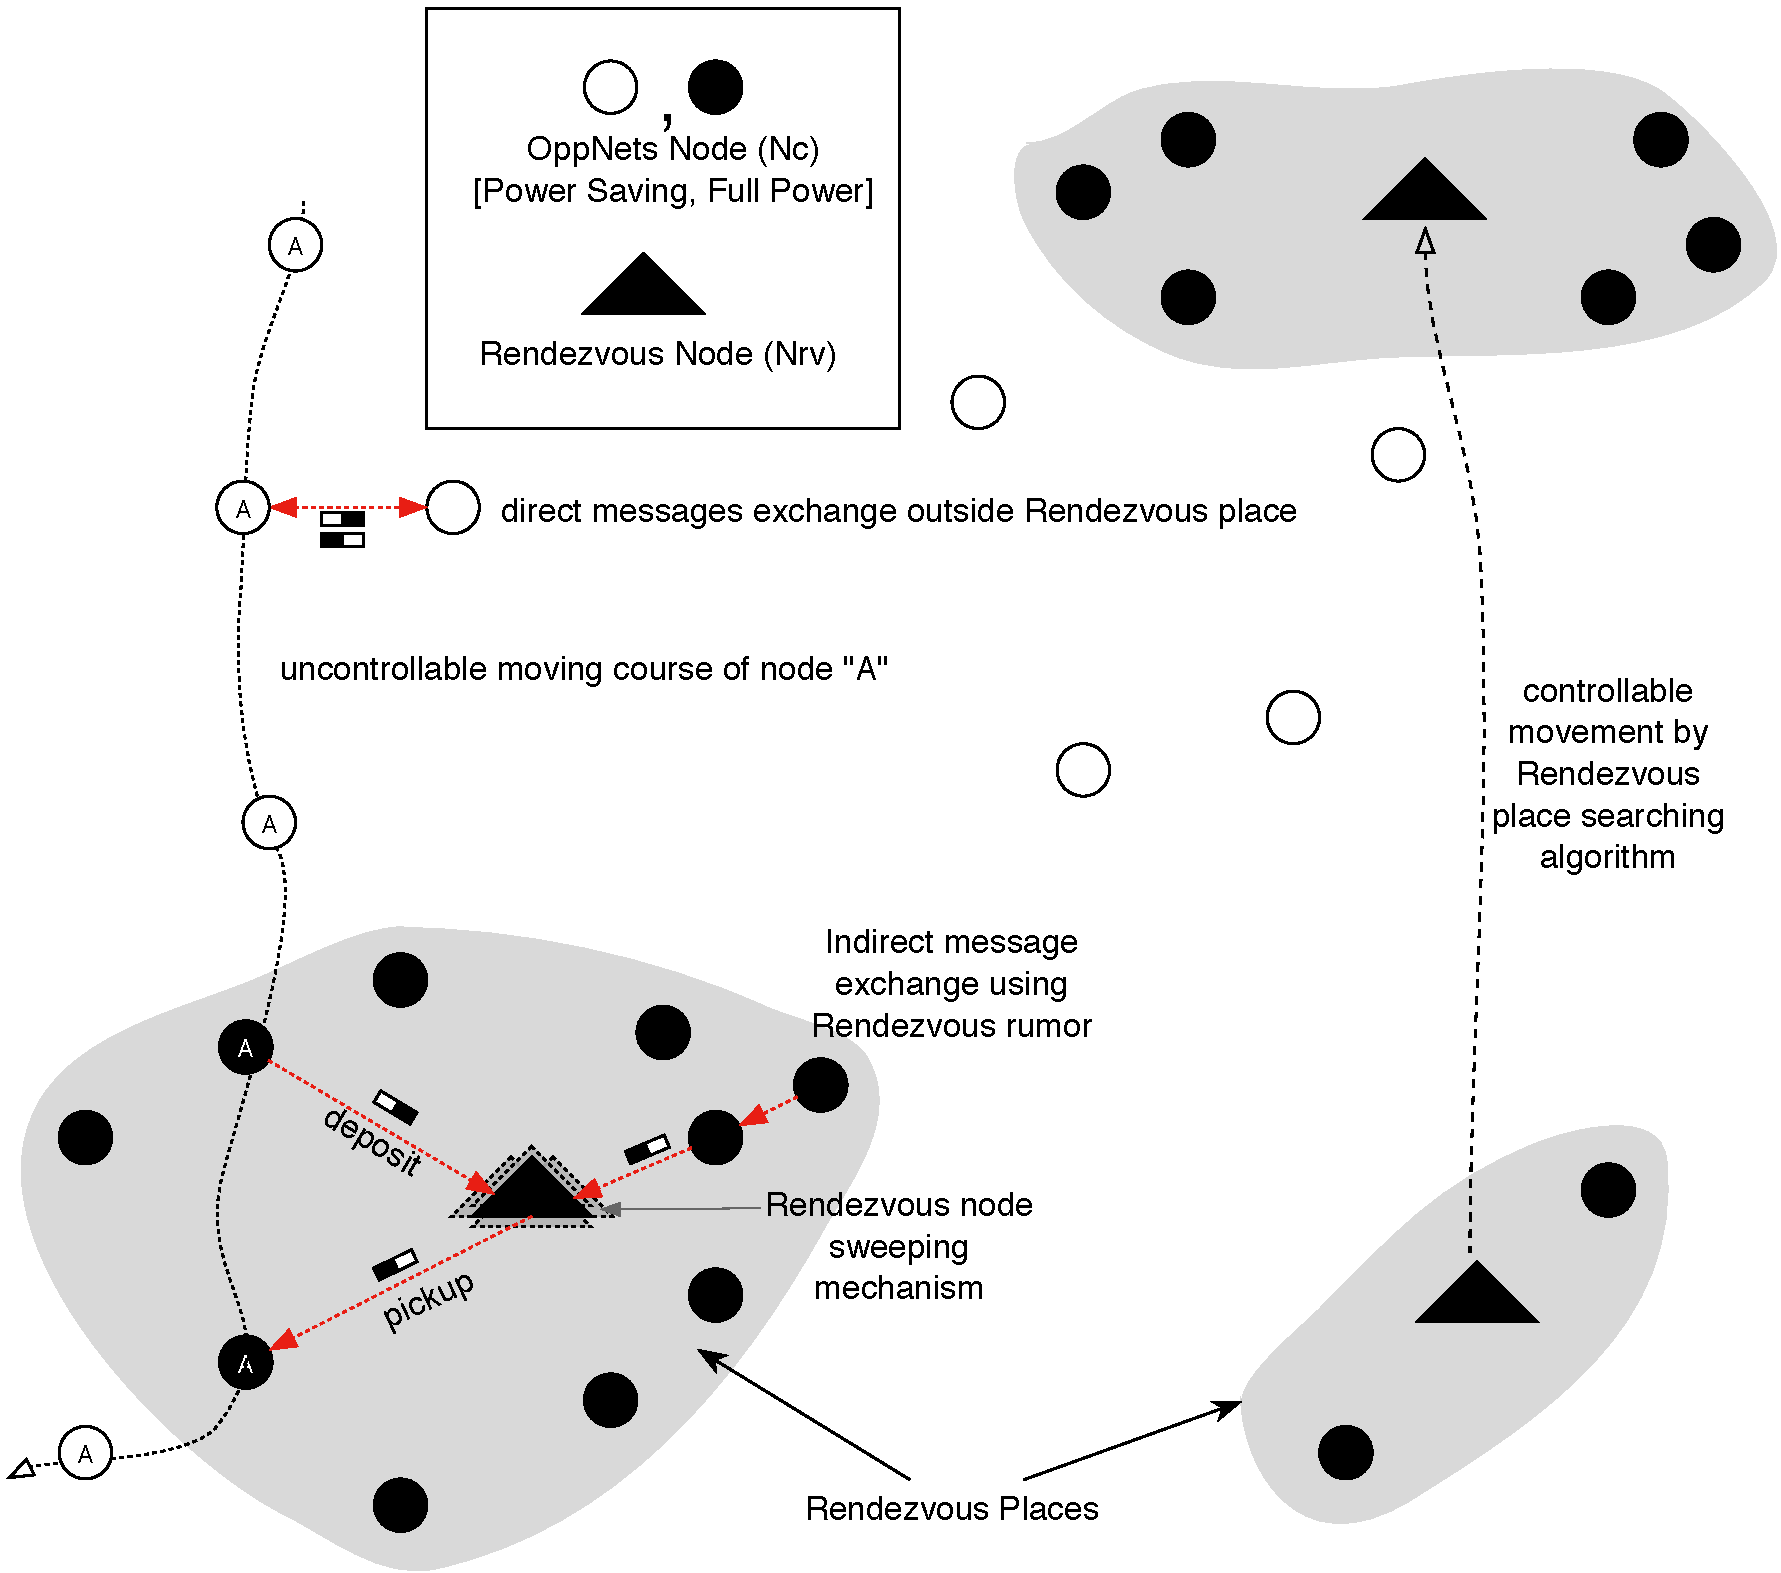
\includegraphics[width=0.7\linewidth]{Figures_Present/NewSystemModel}
\caption{System Model}
\label{fig:NewSystemModel}
\end{figure}
\end{frame}
%------------------------------------------------
\begin{frame}
	\frametitle{OppNet Operation Modes: Full Power \& Power Saving}
	\begin{figure}
\centering
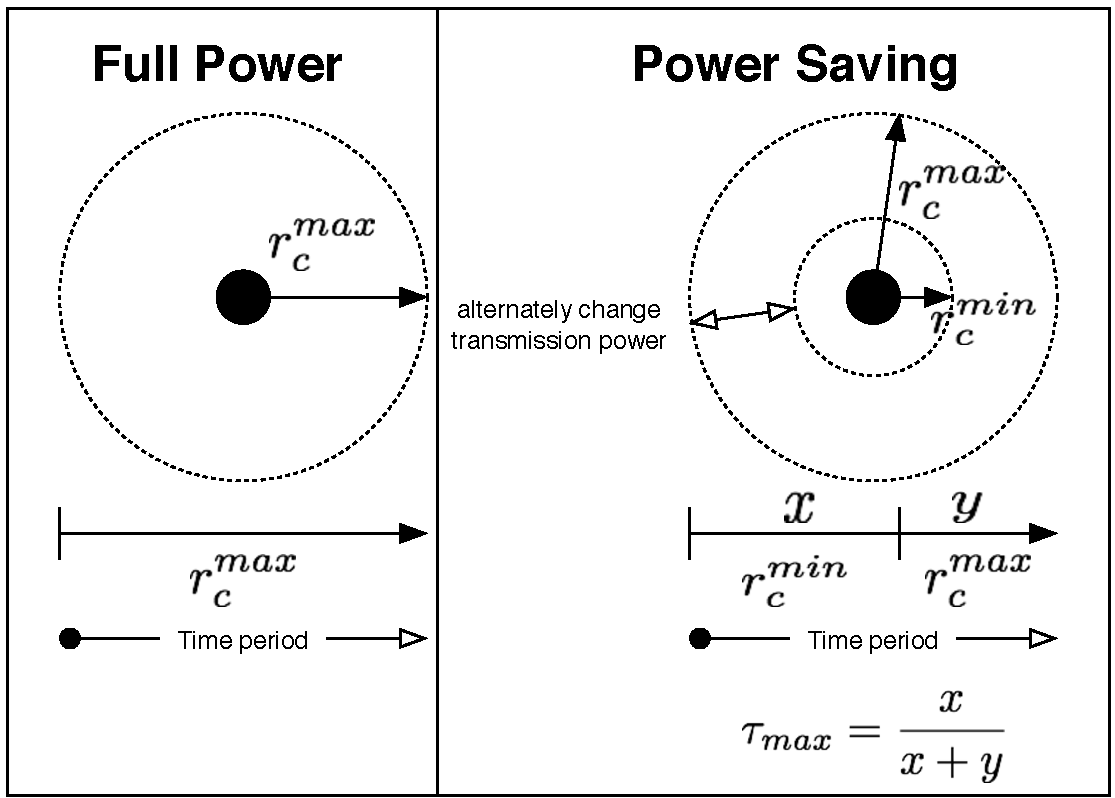
\includegraphics[width=0.7\linewidth]{Figures_Present/OperationalMode}
\caption{Operational Modes}
\label{fig:OperationalMode}
\end{figure}
\end{frame}
%------------------------------------------------
\begin{frame}
	\frametitle{Rendezvous place and its Rumor protocol}
\begin{figure}
\centering
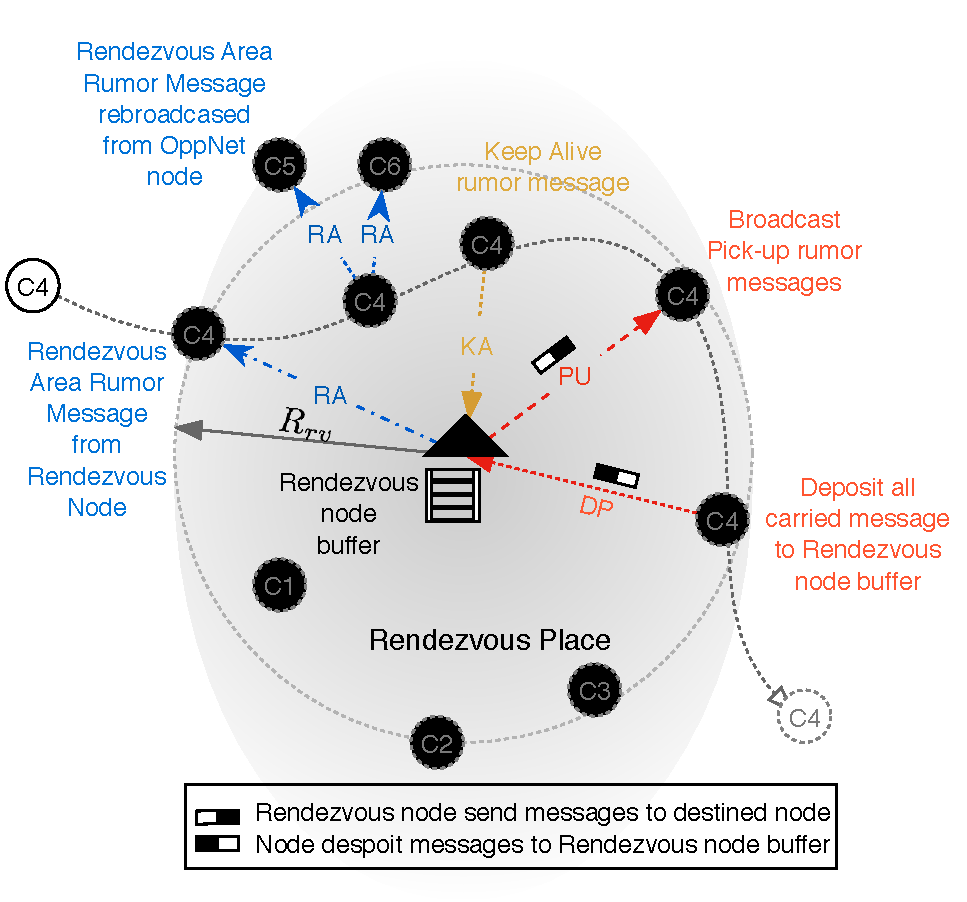
\includegraphics[width=0.7\linewidth]{Figures_Present/NewRendezvousPlace}
\caption{Rendezvous Place}
\label{fig:NewRendezvousPlace}
\end{figure}
\end{frame}
%------------------------------------------------
\begin{frame}
	\frametitle{Rendezvous place searching algorithm}
	\begin{itemize}
		\item Predictable behavior OppNet nodes
		\item Non-Predictable behavior OppNet nodes
	\end{itemize}
\begin{figure}
\centering
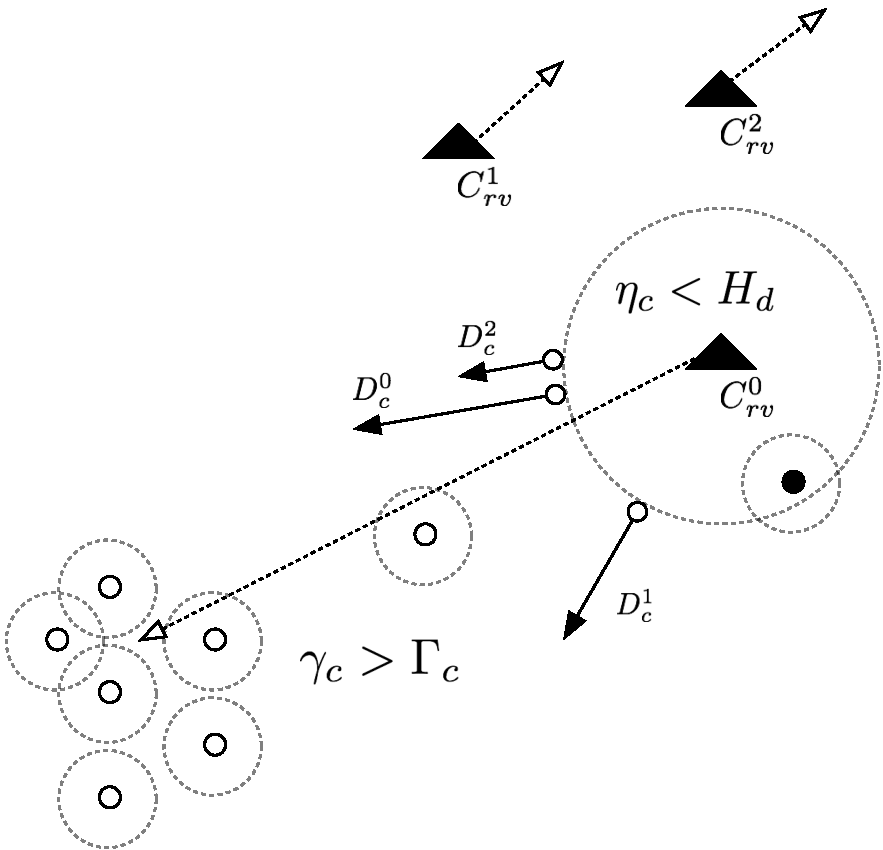
\includegraphics[width=0.5\linewidth]{Figures_Present/Dynamic}
\caption{Rendezvous Place Searching}
\label{fig:Dynamic}
\end{figure}
\end{frame}
%------------------------------------------------
\begin{frame}
	\frametitle{Simulation Setup}
\begin{table}[!t]
	\renewcommand{\arraystretch}{1.3}
	\caption{simulation variables}
	\label{table_parameters}
	\centering
	\begin{tabular}{|c|c|c|c|}
		\hline
		Parameters         & $N_{i}$ & $N_{c}$ & $N_{rv}$ \\ \hline
		Simulation Time     & \multicolumn{3}{|c|}{10800 Seconds }  \\ \hline
		Message Size       &  \multicolumn{3}{|c|}{500 KB - 1 MB}        \\ \hline
		Node Buffer         & \multicolumn{2}{|c|}{500 MB}&  10 GB      \\ \hline
		Radio Range & 30 Meters &  $r_{c} = 30$ Meters  & 100 Meters \\ \hline
		Transmission Speed &  \multicolumn{3}{|c|}{ 54 Mbps   }        \\ \hline
		Router             & \multicolumn{3}{|c|}{ DRRA | Epidemic   } \\ \hline
		Moving Speed       &   \multicolumn{3}{|c|}{0.5 - 1.5 m/s }        \\ \hline
		Movement Model     &   \multicolumn{3}{|c|}{Group Movement Model  }      \\ \hline
	\end{tabular}
\end{table}
\end{frame}
%------------------------------------------------
\begin{frame}
	\frametitle{Simulation Results}
\begin{figure}
\centering
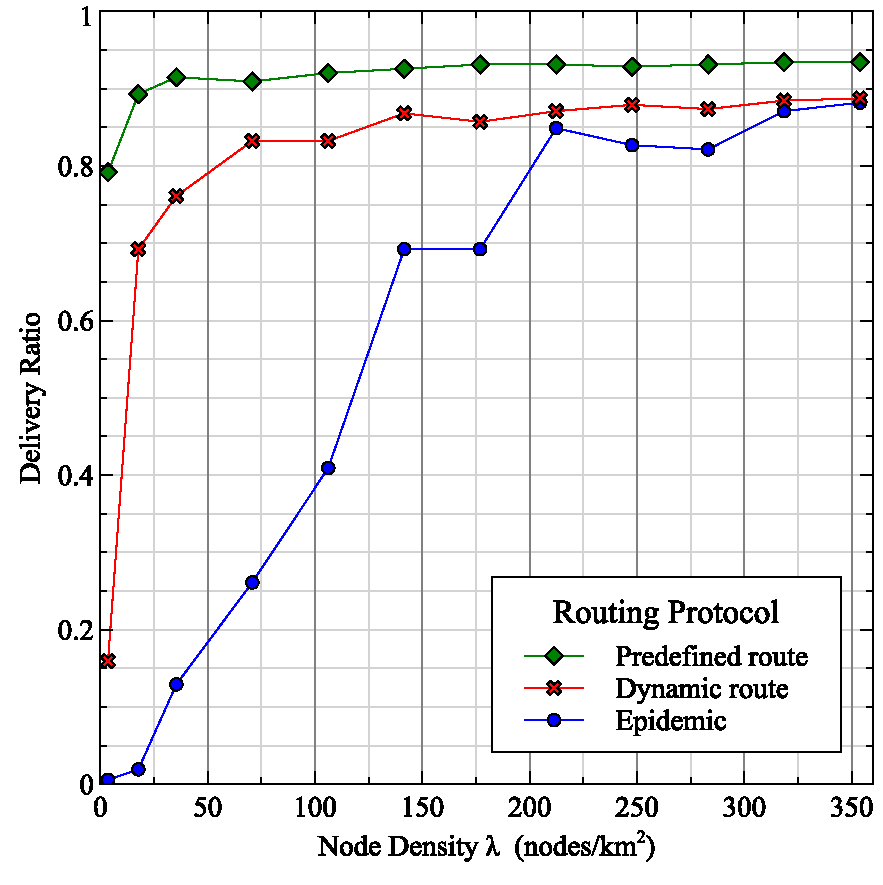
\includegraphics[width=0.6\linewidth]{Figures_Present/DeliveryRatio}
\caption{Delivery Ratio per Node Density}
\label{fig:DeliveryRatio}
\end{figure}
\end{frame}
%------------------------------------------------
\begin{frame}
	\frametitle{Simulation Results}
	\begin{figure}
		\centering
		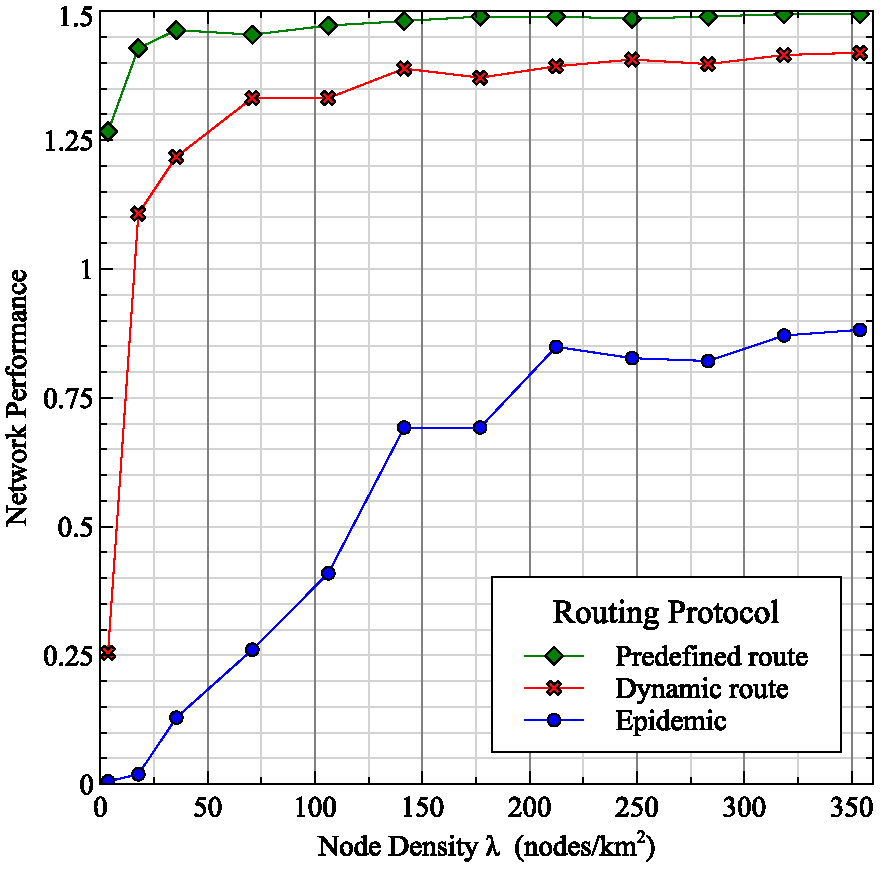
\includegraphics[width=0.6\linewidth]{Figures_Present/NetworkPerformance}
		\caption{Network Performance per Node Density}
		\label{fig:NetworkPerformance}
	\end{figure}
\end{frame}
%------------------------------------------------
%------------------------------------------------
\begin{frame}
	\frametitle{Simulation Results}
\begin{figure}
\centering
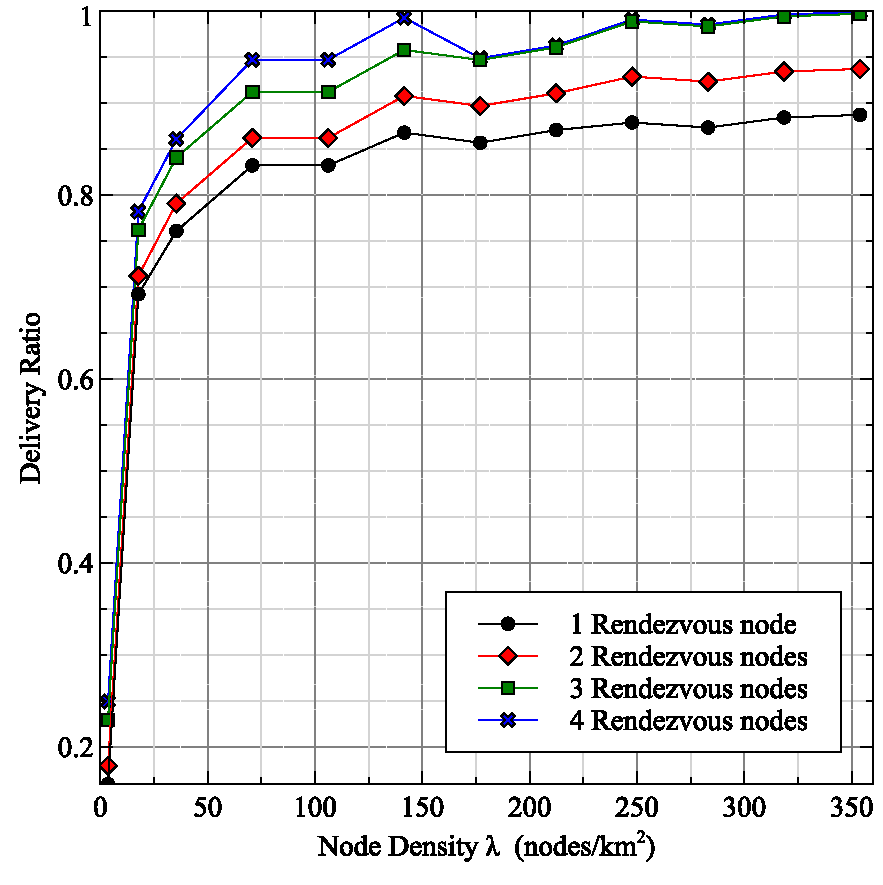
\includegraphics[width=0.6\linewidth]{Figures_Present/MultipleRVs}
\caption{Multiple Rendezvous Places}
\label{fig:MultipleRVs}
\end{figure}
\end{frame}
%------------------------------------------------
%------------------------------------------------
\begin{frame}
	\frametitle{Simulation Results}
\begin{figure}
\centering
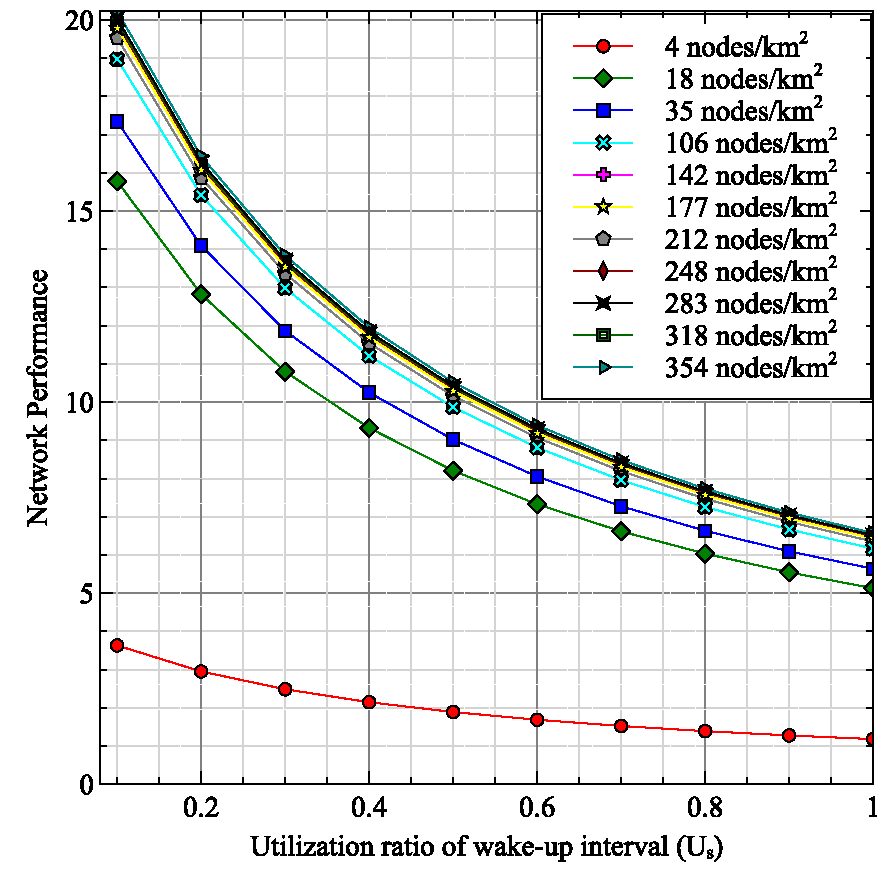
\includegraphics[width=0.6\linewidth]{Figures_Present/Utilization}
\caption{Network Performance per Utilization Ratio}
\label{fig:Utilization}
\end{figure}
\end{frame}
%------------------------------------------------
%------------------------------------------------
\begin{frame}
	\frametitle{Conclusion}
\begin{itemize}
	\item Our protocols perform significant higher in network network performance which is the tradeoff of delivery ratio per energy consumption. 
	\item If the location of rendezvous can be predefined, we can achieve highest network performance. 
	\item The carried node can gain higher network performance if the sleep mode is longer than awake mode.
\end{itemize}
\end{frame}
%------------------------------------------------
%------------------------------------------------
\section{Data-wise Opportunistic Routing with Spatial Information}
%------------------------------------------------
\begin{frame}
	\frametitle{DORSI Routing Algorithm}
	\begin{figure}
\centering
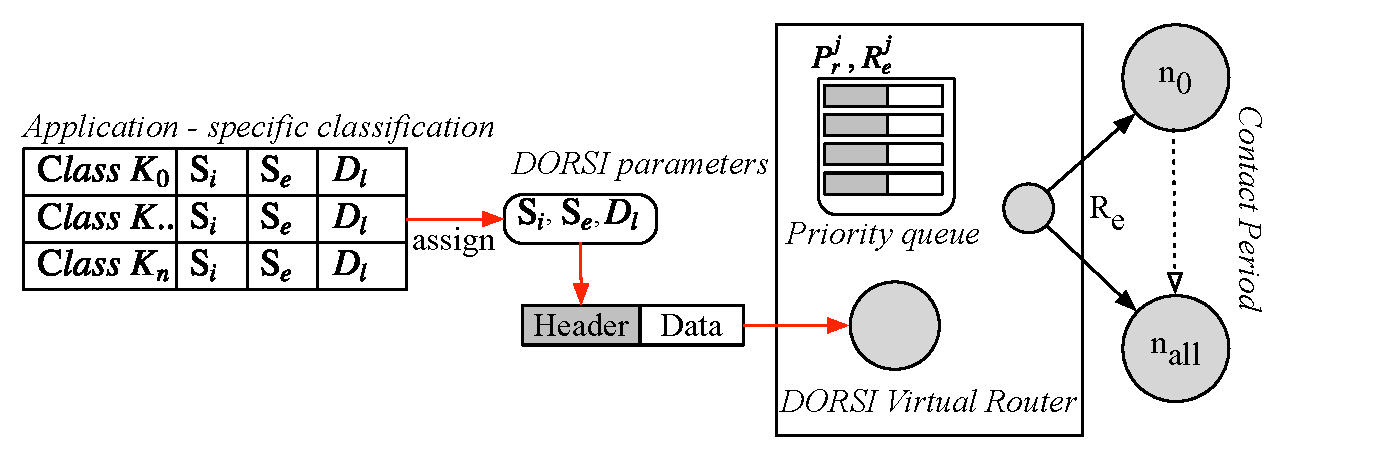
\includegraphics[width=0.7\linewidth]{Figures_Present/Fig2}
\caption{DORSI System Model}
\label{fig:Fig2}
\end{figure}
\end{frame}
\begin{frame}
	\frametitle{DORSI Routing Algorithm}
\begin{eqnarray}
{ P }_{ r }^{ j }={ w }_{ p }{ S }_{ i }^{ j }+(1-{ w }_{ p })\xi ({ D }_{ l }^{ j },t)
\end{eqnarray}
where
$ \xi ({ D }_{ l }^{ j },t)=\begin{cases} 0;{ \tau  }_{ t }>{ \tau  }_{ max } \\ \frac { { \tau  }_{ max }-{ \tau  }_{ t } }{ { \tau  }_{ max }-{ \tau  }_{ min } }  \\ 1;{ \tau  }_{ t }<{ \tau  }_{ max } \end{cases};{ \tau  }_{ min }\le { \tau  }_{ t }\le { \tau  }_{ max } $
\begin{eqnarray}
{ R }_{ e }^{ j }=(1-{ R }_{ min })[{ w }_{ r }{ P }_{ r }+(1-{ w }_{ r })(1-{ S }_{ e }^{ j })]+{ R }_{ min }
\end{eqnarray}
\end{frame}

%--------------
%------------------------------------------------
\begin{frame}
	\frametitle{Node Ranking Model}
\begin{figure}
\centering
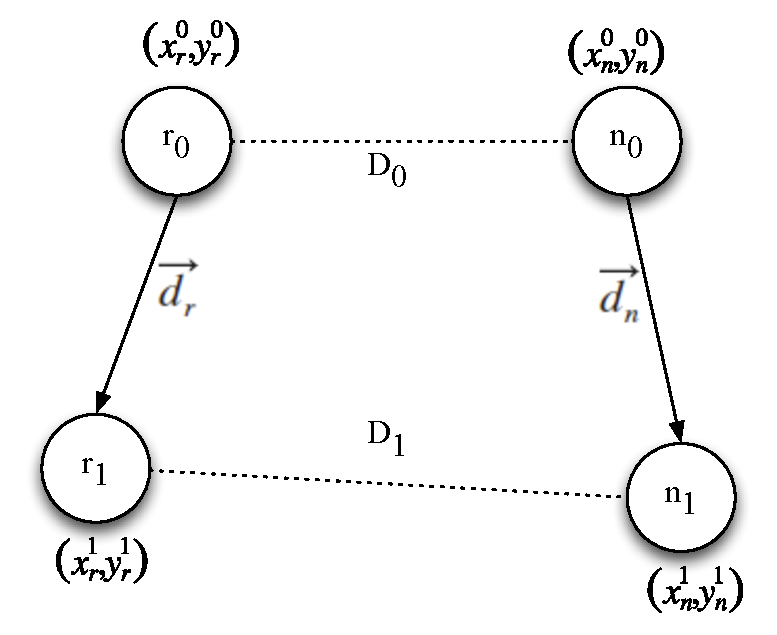
\includegraphics[width=0.5\linewidth]{Figures_Present/Fig3}
\caption{Node Ranking Model}
\label{fig:Fig3}
\end{figure}
{\tiny \begin{eqnarray}
{ N }_{ r }^{ n }=\sqrt { { ({ x }_{ n }\cos { { \theta  }_{ n } } -{ x }_{ r }^{ t }\cos { { \theta  }_{ r }^{ t } } ) }^{ 2 }-{ ({ y }_{ n }\sin { { \theta  }_{ n } } -{ x }_{ r }^{ t }\sin { { \theta  }_{ r }^{ t } } ) }^{ 2 } } -\sqrt { { ({ x }_{ n }-{ x }_{ r }^{ t }) }^{ 2 }-{ ({ y }_{ n }-{ x }_{ r }^{ t }) }^{ 2 } } 
\end{eqnarray}}
\end{frame}
%------------------------------------------------
\begin{frame}
	\frametitle{Evaluation}
	\begin{table}[!t]
		\renewcommand{\arraystretch}{1.3}
		%\caption{simulation variables}
		%\label{table_parameters}
		\centering
		\begin{tabular}{|c|c|c|}
			\hline
			Parameters         & DORSI                  & Epidemic \\ \hline
			Operation Time     & \multicolumn{2}{|c|}{3600 Seconds }  \\ \hline
			Message Size       &           \multicolumn{2}{|c|}{500 KB - 5 MB}        \\ \hline
			Node Buffer        &              \multicolumn{2}{|c|}{1000 MB   }       \\ \hline
			Transmission Range &              \multicolumn{2}{|c|}{150 Meters  }        \\ \hline
			Transmission Speed &              \multicolumn{2}{|c|}{ 54 Mbps   }        \\ \hline
			Node Density       &                \multicolumn{2}{|c|}{0 - 100 \% }        \\ \hline
			Router             & DORSI                  & Epidemic \\ \hline
			Deadline                &  \multicolumn{2}{|c|}{Relative to data class}       \\ \hline
			Moving Speed       &          \multicolumn{2}{|c|}{0.5 - 1.5 m/s }        \\ \hline
			Movement Model     &       \multicolumn{2}{|c|}{Random Waypoint  }      \\ \hline
			Wait Time     &       \multicolumn{2}{|c|}{0 - 180 Seconds  }      \\ \hline
		%	Number of classes     &       \multicolumn{2}{|c|}{5 }      \\ \hline
		\end{tabular}
	\end{table}
\end{frame}
%------------------------------------------------
\begin{frame}
	\frametitle{Simulation Results}
\begin{figure}
\centering
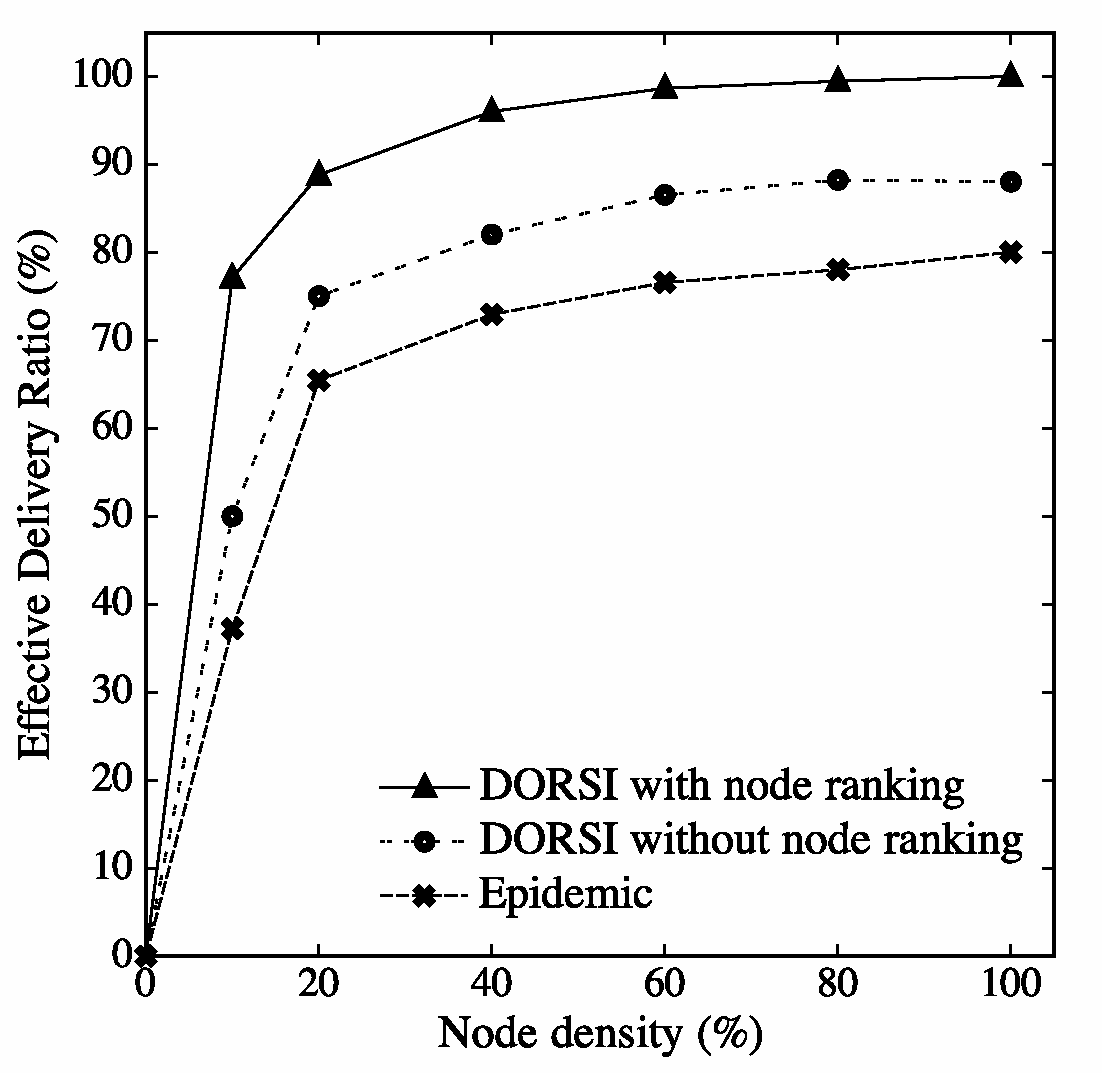
\includegraphics[width=0.5\linewidth]{Figures_Present/Fig4-eps-converted-to}
\caption{Effective Delivery Ratio per Node Density}
\label{fig:Fig4-eps-converted-to}
\end{figure}
\end{frame}
%------------------------------------------------
\begin{frame}
	\frametitle{Simulation Results}
\begin{figure}
\centering
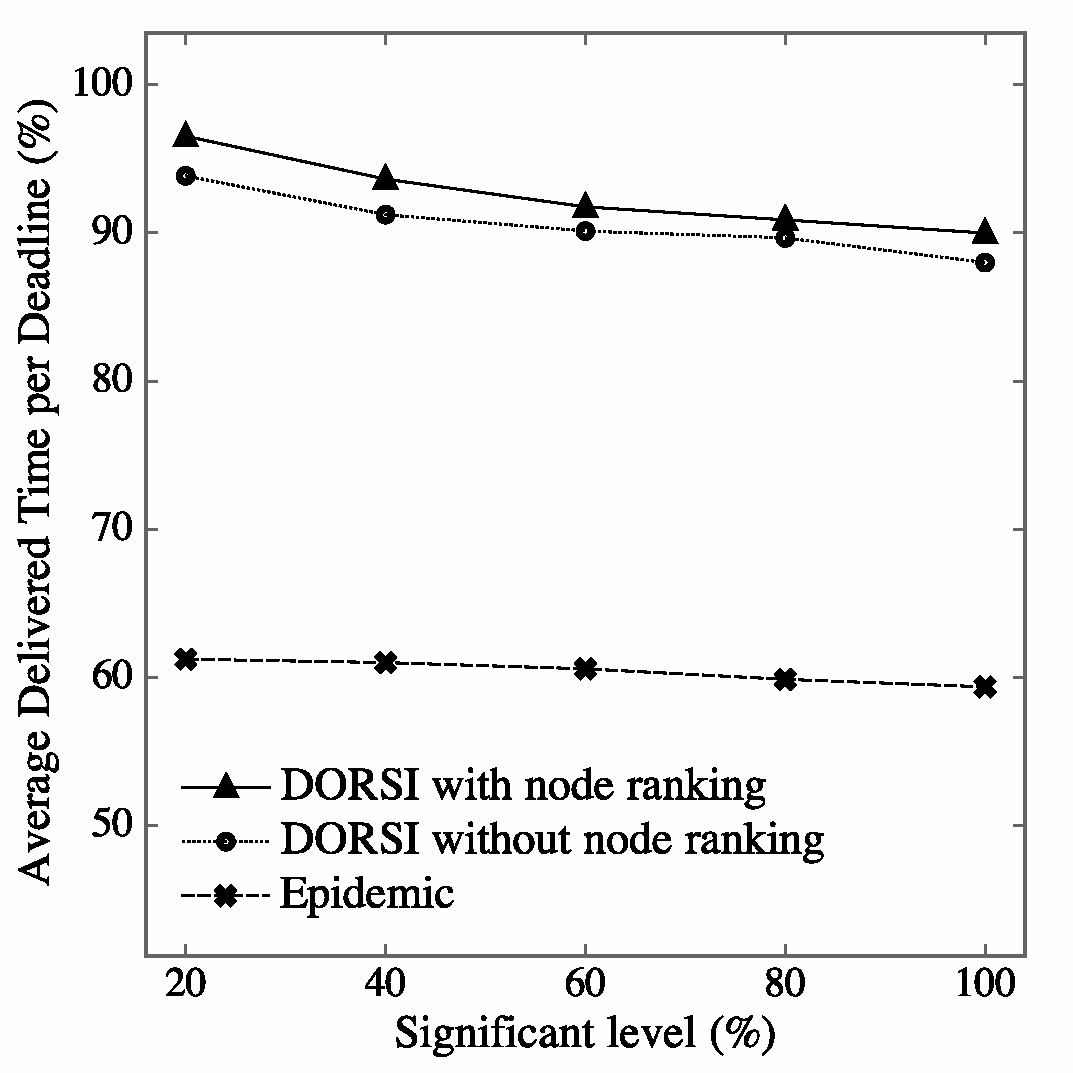
\includegraphics[width=0.5\linewidth]{Figures_Present/Fig5-eps-converted-to}
\caption{Average Delivered Time per Deadline on Significant Level}
\label{fig:Fig5-eps-converted-to}
\end{figure}
\end{frame}
%------------------------------------------------
\begin{frame}
	\frametitle{Simulation Results}
\begin{figure}
\centering
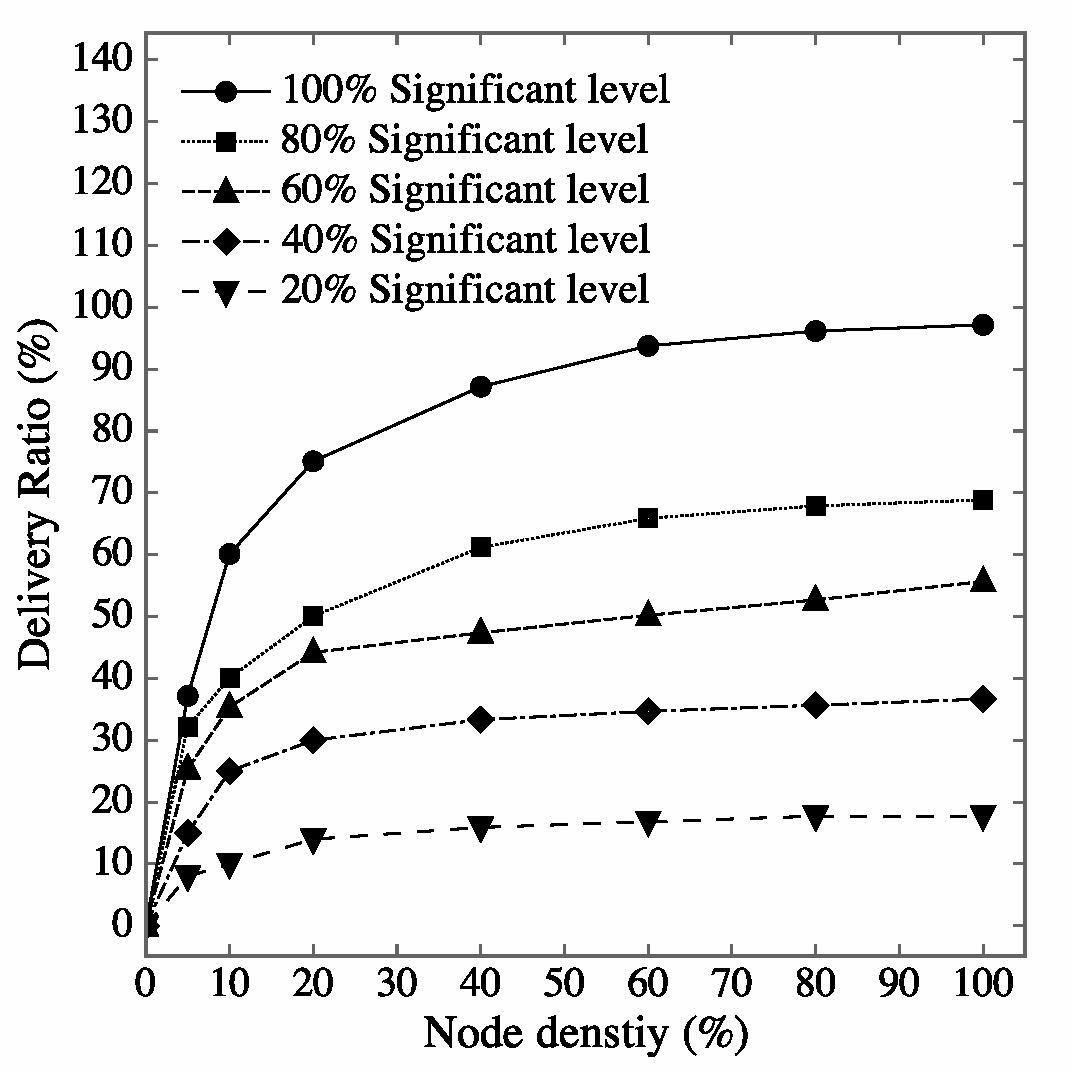
\includegraphics[width=0.5\linewidth]{Figures_Present/Fig6-eps-converted-to}
\caption{DORSI Delivery Ratio on each class}
\label{fig:Fig6-eps-converted-to}
\end{figure}
\end{frame}
%------------------------------------------------
\begin{frame}
	\frametitle{Simulation Results}
\begin{figure}
\centering
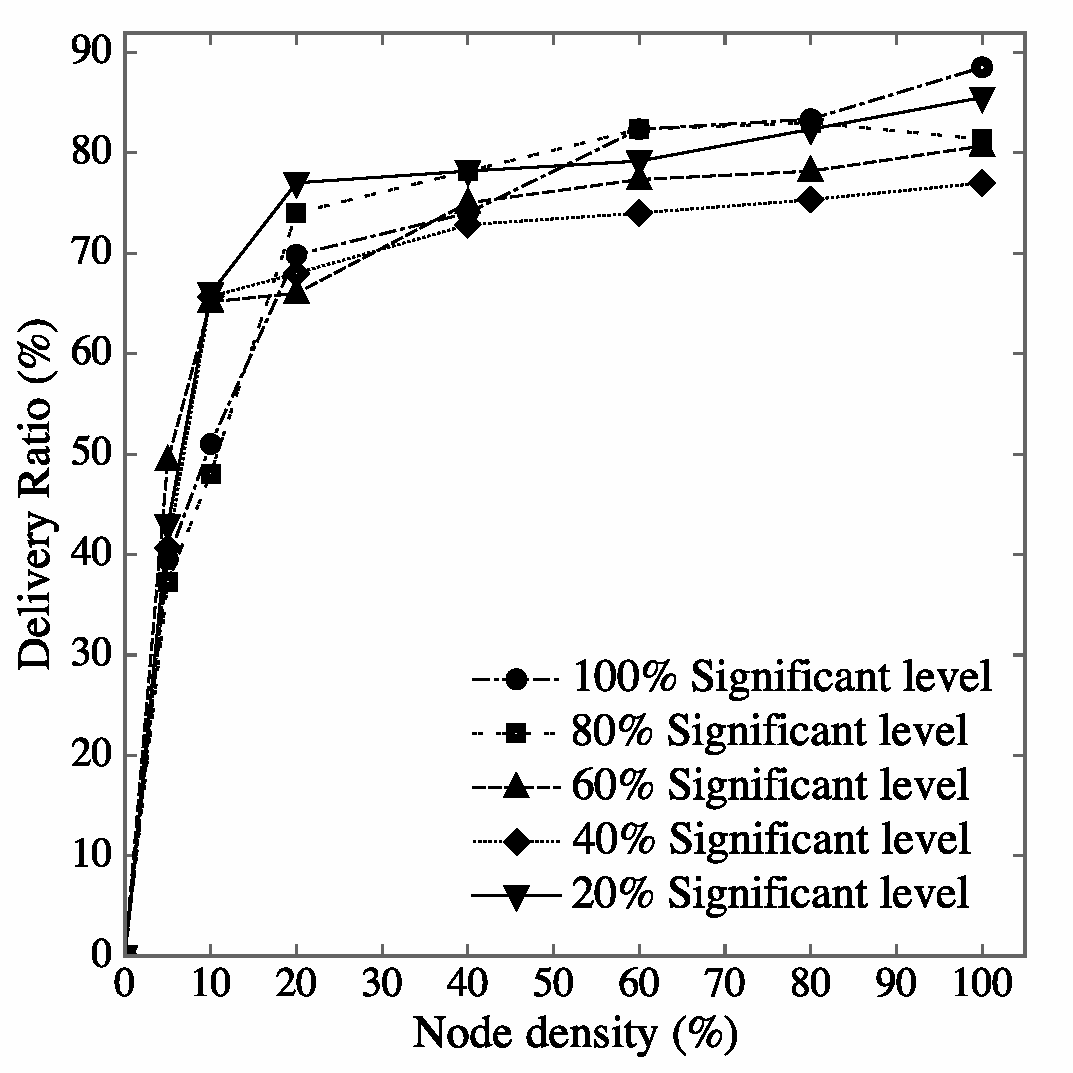
\includegraphics[width=0.5\linewidth]{Figures_Present/Fig7-eps-converted-to}
\caption{Epidemic Delivery Ratio on each class}
\label{fig:Fig7-eps-converted-to}
\end{figure}
\end{frame}
%------------------------------------------------
\begin{frame}
	\frametitle{Simulation Results}
\begin{figure}
\centering
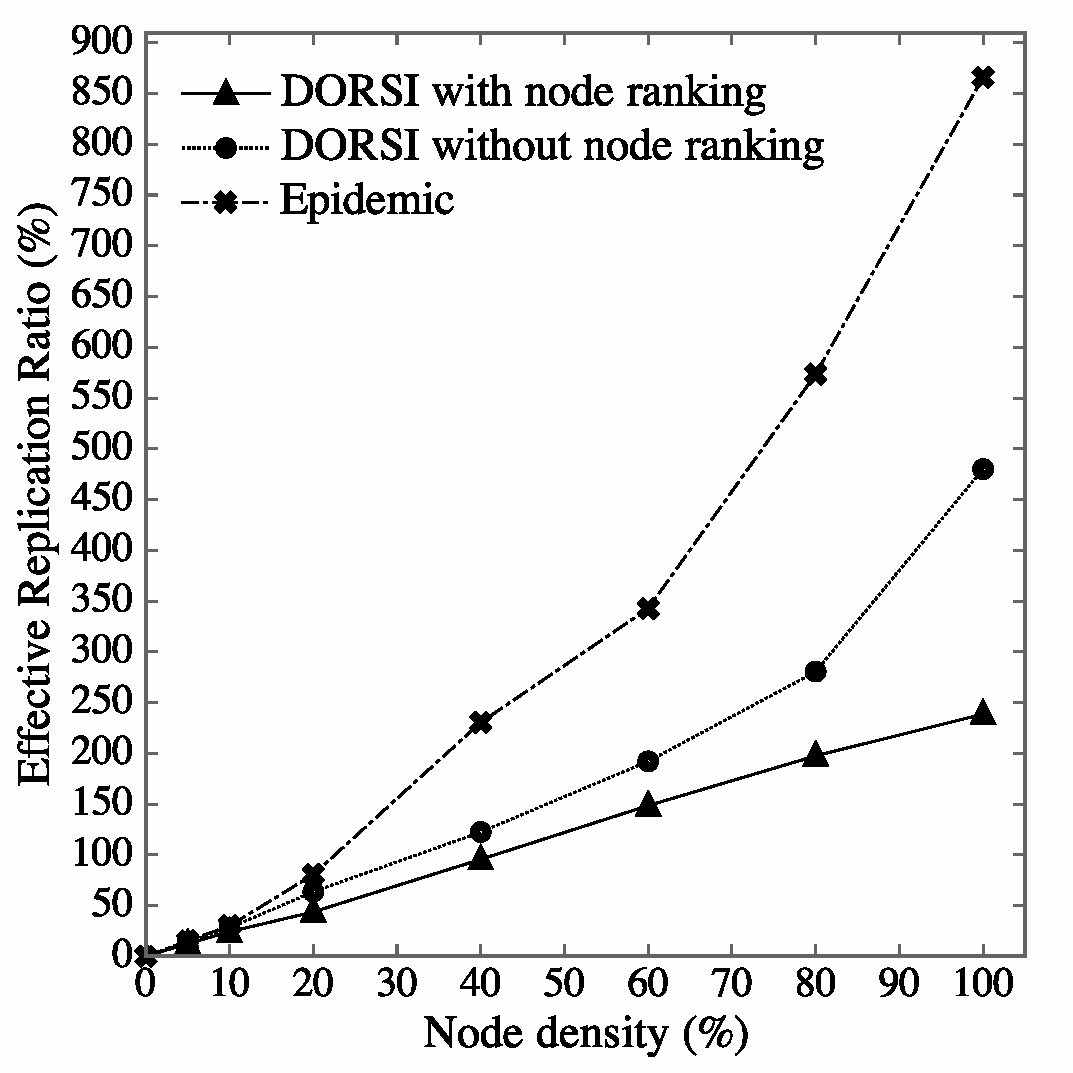
\includegraphics[width=0.5\linewidth]{Figures_Present/Fig8-eps-converted-to}
\caption{Effective Replication Ration Comparison}
\label{fig:Fig8-eps-converted-to}
\end{figure}
\end{frame}
%------------------------------------------------
\begin{frame}
	\frametitle{Simulation Results}
\begin{figure}
\centering
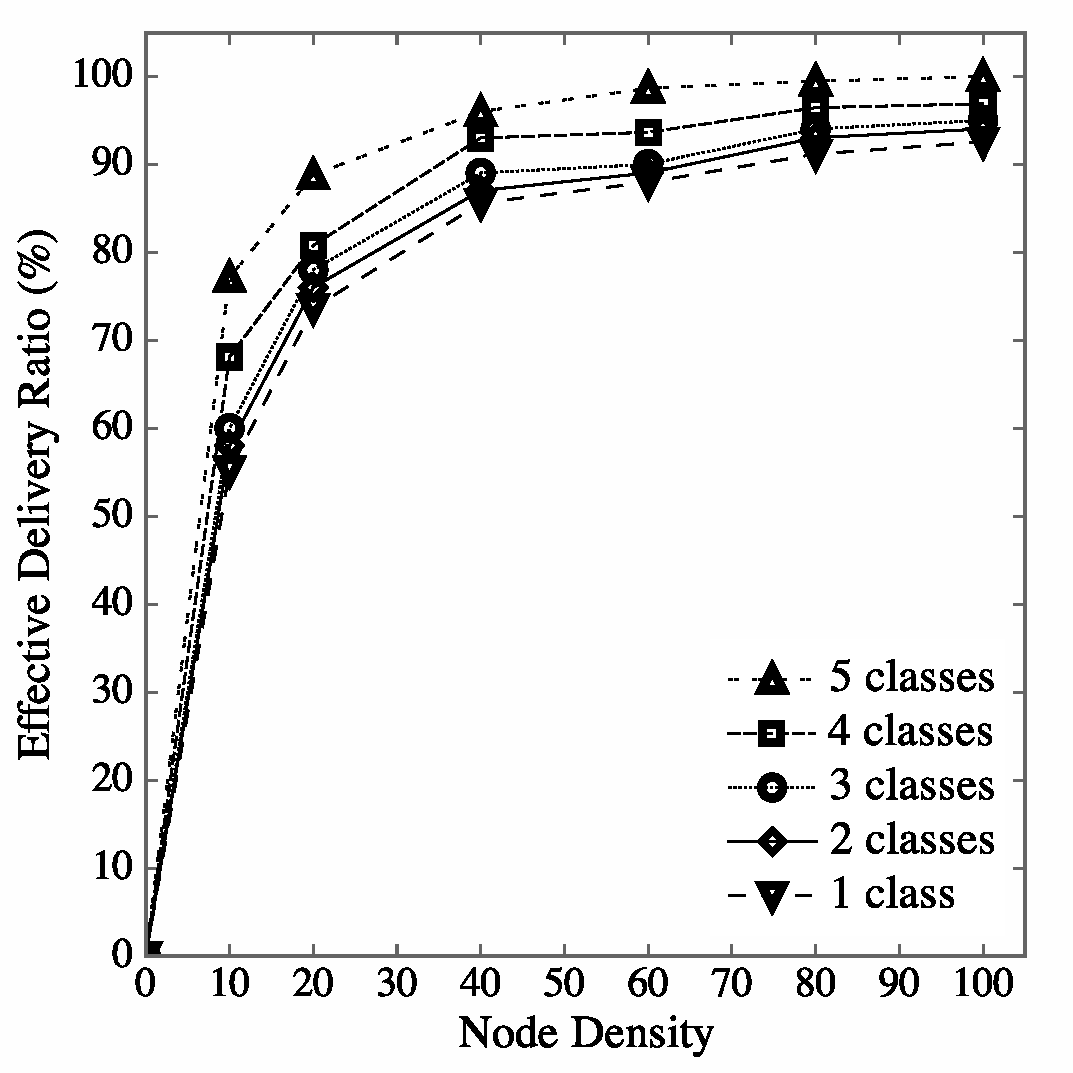
\includegraphics[width=0.5\linewidth]{Figures_Present/Fig9-eps-converted-to}
\caption{EDR on different classification scale}
\label{fig:Fig9-eps-converted-to}
\end{figure}
\end{frame}
%------------------------------------------------
\begin{frame}
	\frametitle{Conclusion}
	\begin{itemize}
		\item Two key performance indexes (1) effective delivery ratio and (2) effective replication ratio: remarkably improve over the traditional Epidemic routing. 
		\item Delivery ratio of DORSI and Epidemic comparison shows notable overall enhancement of the network routing efficiency. \item DORSI protocol can guarantee higher delivery ratio on more important data while limiting the replication of data with higher security level. 
		
		%The average delivered time of DORSI also shows the optimal bandwidth utilization since it can control the messages to reach the destination closer to their deadline. In addition, this method can be applied to different scale of data classification to suit any application deployment. Furthermore, our work can be extended in various directions. An obvious extension of the work could be the evaluation of our approach on a virtualization network to physically obtain the real life results comparing to the results from this simulation result. Next, we will evaluate the performance of our method in different conditions in order to apply data classification routing technique on more general applications.
	\end{itemize}
	
\end{frame}
%------------------------------------------------
\section{Conclusion }
%------------------------------------------------
\begin{frame}
	\frametitle{Conclusion }
	\begin{itemize}
		\item With these two novel proposed OppNet routing algorithms, the delivery ratio of network can be improved especially on the sparse network environment
		\item Rendezvous based routing can optimize the power utilization among mobile nodes.
		\item DORSI can improve the deliverable of important messages thus the network gains higher delivery ratio
	\end{itemize}
	
\end{frame}


\begin{frame}
\frametitle{References}
\footnotesize{

\bibliography{ref}

}
\end{frame}
\end{document}
